\documentclass[a4paper, 12pt]{article}
\usepackage{setspace}
\usepackage{graphicx}
\usepackage{longtable}
\usepackage[backend=bibtex,style=numeric]{biblatex}
\usepackage{mathtools}
\addbibresource{bibliography.bib} 
\graphicspath{ {images/} }
\doublespacing

\begin{document}
\title{Using Machine Learning For DOTA2 Match Prediction}
\author{Andrius Buinovskij}
\maketitle

    \section{Dictionary}

	\par There are some more obscure terms littered throughout the text. Here is a short explanation for each one.

        \begin{itemize}
            \item A \textbf{feature} is some aspect of something. For instance, a coin may have a mass, an area, an average colour and so on. Each of those are a feature.
            \item \textbf{Classification} is the problem of identifying to which of a set of categories (sub-populations) a new observation belongs, on the basis of a training set of data containing observations (or instances) whose category membership is known.\footnote{Wikipedia.}

        \end{itemize}

    \section{Introduction}

        \par This text describes four contemporary machine learning techniques, and then shows their application in match outcome prediction in a game of Dota 2, namely, which team will win, based on players' hero selection. In other words, it is classifying team composition as preferring a radiant win, or preferring a dire win.

        \par The game in question, Defence of the Ancients (DOTA) 2, is very nuanced and has a plethora of mechanics. For the purposes of this paper however, it will suffice to say that in a game of DOTA, two teams, "Dire" and "Radiant"\footnote{Dire being evil and red, Radiant being green good.}, five players per team, try to destroy the other team's base. At the beginning of a game, each player chooses a "hero" to play, a character within the game. Different heroes have different abilities, and some heroes synergize, whilst others cancel each other out. As of writing of this text, there are 113 different heroes, resulting in a bewildering number of possible team compositions.
        
    \newpage

    \section{Background}

        \par The machine learning techniques used are: Nearest Neighbours, Neural Networks, Support Vector Machines and Boosting.
        
        \subsection{Machine Learning Generalities}
        
            \par In general, the (supervised, since this is what this particular project is about) machine learning pipeline looks something like this:
            
                \begin{figure}[h]
                    \caption{General machine learning process.}
                    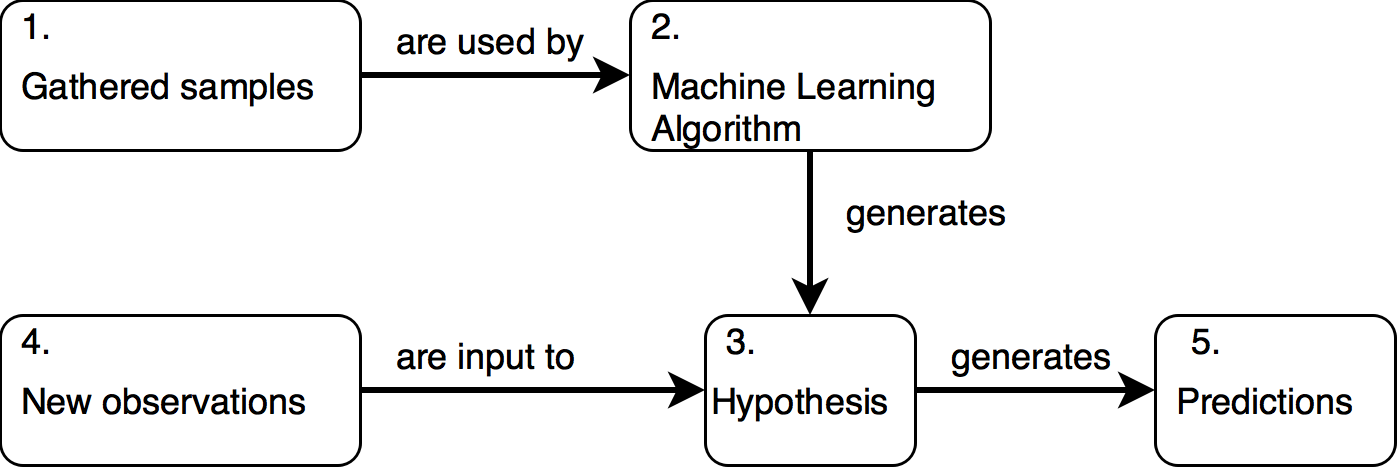
\includegraphics[width=\textwidth]{machineLearningGeneralNotion}
                \end{figure}
                
            \par We begin with some dataset of examples. This could be a list of coins, their value and their mass, or it could be a list of houses and their square footage, number of bedrooms, the price they sold for and so forth. The dataset will be split into the data, and "the label", which will be the feature the algorithm will try to learn about. 
            
            \par Then we pass this dataset to the machine learning algorithm. The algorithm will "train" a model, called a hypothesis for historical reasons, basically adjusting parameters of the model such that the model will perform as well as possible on the dataset, which will hopefully generalize to out-of-sample performance. 
            
            \par What is meant by performance is that, in classification, each sample will belong to some category. The more of the training sample the algorithm classifies correctly, the better is it's in-sample performance. This could be, given the square footage and number of bedrooms of a house, predict whether it is worth more than 500,000 Euro. The algorithm is trained such that it will classify correctly as many training samples as possible.
            
            \par This trained model or hypothesis will then be able to take some new observations, perhaps a new coin or a house description, and predict the label.
            
            \par The hypothesis is formed using the training set, but is validated using a testing set. This means that the hypothesis is tested on a set of samples that it was not trained on to see how well the hypothesis will perform in the "real world", or how well it will "generalize" to out-of-training set samples.
            
            \par For a more in-depth explanation, please see\cite{machineLearningBackground}.

        \subsection{Nearest Neighbours}

            \subsubsection{Nearest Neighbours Intuition}

                \par The simple logic behind the nearest neighbours approach to machine learning is: when asked to classify a new observation, one should see if the scenario in question has occurred before within the training set, and see what was done then. If the precise scenario has not occurred, then one should find the most similar scenario on record for guidance.

                \par Let us say that we are trying to build an algorithm which will be used as a part of vending machines, namely, deciding on the value of coins that are inserted into the machine. Let us also say that the value of the coin will be decided based solely on it's mass (for simplicity), and that we have a training set of coins already weighed and labelled.

                \par A coin is inserted into the vending machine, how can we tell it's precise value? All we have to go by is the coin's mass. Currently, our training set is illustrated below.

                \begin{figure}[h]
                    \caption{A visualization of coins placed on mass axis.}
                    \centering
                    \includegraphics[width=\textwidth]{coinAxis}
                \end{figure}
                

                \par So we have three coins of mass of 2, 5 and 10 grams. Let us say a coin is inserted into the machine, of mass of 6 grams. Here it is on our graph.

                \begin{figure}[h]
                    \caption{Coin graph including mismatching coin.}
                    \centering
                    \includegraphics[width=\textwidth]{coinAxis2}
                \end{figure}

                \par We would like to decipher the value of the newly inserted coin. An immediately obvious approach is to query our training set of already known mass-value pairs of coins to find a coin that most closely resembles the new coin, and say that the two are the same. Within the graph, this is simply looking for the nearest neighbouring coin\footnote{Hence the name of the method, Nearest Neighbours.}. Here it is again on our graph.

                \begin{figure}[h]
                    \caption{The nearest neighbour to the unknown coin}
                    \centering
                    \includegraphics[width=\textwidth]{nearestNeighbour}
                \end{figure}

                \par Having found the nearest neighbour, the 20 cent coin, we conclude that the new coin must also be a 20 cent coin, perhaps with some imperfections.

                \par This short example illustrates the benefits and shortcomings of Nearest Neighbours. The method is simple and logical, and directly uses experience of the past. However, it is not extracting underlying patterns out from underneath the data, but is instead simply\footnote{Not for long.} looking to the past for similar cases.
                
            \newpage


            \subsubsection{Adding complexity and Trees}

                \par Our coin example was quite simple, using a single feature, and just three neighbour entries. A single feature gives rise to a single axis, however, we could have used more. For instance, we could have used the coin's area, which would have looked like the following:
                
                \begin{figure}[h]
                    \caption{A visualization of coins places on area and mass axes}
                    \centering
                    \includegraphics[width=\textwidth]{twoAxes}
                \end{figure}

                \par The search for a nearest neighbour is now a two-dimensional one, which we can still handle intuitively. However, as the number of features, and consequently axes, grows, the question of how does one find nearest neighbours arises.

                \par So, how does one find the nearest neighbours, and do so efficiently? Presented are three algorithms.
                
                
                \subsubsection{Brute force}
                
                    \par Let the set of exemplar coins (the 10, 20 and 50 cent coins) be \textbf{S} and the newly observed coin be \textbf{T}. 
                    
                    \par The brute force approach to finding k number of nearest neighbours is to simply calculate the distance\footnote{Preferably a non-negative, symmetric and satisfying the triangle inequality function.} between \textbf{T} and every member of \textbf{S}, and keep the k nearest neighbours.
                    
                    \par Unfortunately, this method has a running time of \textit{O(ckn)}\footnote{or, less a less naive cn}, where c is the cost of calculating the distance function, k is the number of nearest neighbours desired and n is the number of exemplars in the set \textbf{S}.
                    
                \subsubsection{Kd-trees}
                
                    \par The idea behind kd-trees is to build a tree structure to segment the set \textbf{S} such that to find the nearest neighbours, one only has to examine one of those segments\footnote{Not quite, more on that later}. This is similar to how a human would look for a nearest neighbour on a graph. Instead of checking every point, no matter how far away on the graph, we would focus our attention on the nearby points, since the far away points are irrelevant.
                    
                    \newpage
                    
                    \par Here is a new set of exemplars \textbf{S}, to better demonstrate the algorithm.
                    
                    \begin{center}
                        \begin{tabular}{| l | l | l | l |}
                            \hline
                            Id & Feature A & Feature B & Feature C \\ \hline
                            0 & 2 & 8 & 4 \\ \hline
                            1 & 1 & 4 & 3 \\ \hline
                            2 & 3 & 5 & 7 \\ \hline
                            3 & 10 & 2 & 3 \\ \hline
                            4 & 2 & 12 & 1 \\ \hline
                            5 & 7 & 4 & 8 \\ \hline
                            6 & 5 & 4 & 9 \\ \hline
                            7 & 2 & 7 & 1 \\ \hline
                             
                        \end{tabular}  
                    \end{center}                
                    
                    \par Each row corresponds to a single exemplar, where the exemplars have three features each, namely A, B, and C.
                    
                    \par Now we are going to split \textbf{S} in two. A question arises of how to best do this. The answer is to pick the feature with the largest variance, and then choose the median value from the current set of exemplars being split.\cite{kNearestNeighbours}\footnote{The reasoning is explained under "The Optimized k-d Tree", page 7.}
                    
                    \newpage
                    
                    \par On the first pass through, the feature with the greatest variance is B. Now we choose the median value, which in this case is 4.5 (4+5/2, even numbers). So now all exemplars which have a value of B which is less than or equal to this median go to the left branch, whilst all greater than 4.5 go to the right branch, as follows:
                    
                    \begin{figure}[h]
                        \caption{A visualization of the first segmentation.}
                        \centering
                        \includegraphics[width=\textwidth]{kdTreeFirstDivision}
                    \end{figure}
                    
                    \newpage
                    
                    \par Now we do this again on both children nodes of the root. On the left-hand node, the feature with the greatest variance is A, and the median is 6. On the right-hand node, the feature with the greatest variance is B, and the median is 7.5. This is the result:
                    
                    \begin{figure}[h]
                        \caption{A visualization of the second segmentation.}
                        \centering
                        \includegraphics[width=\textwidth]{kdTreeSecondDivision}
                    \end{figure}
                    
                    \newpage
                    
                    \par Now the tree is 2 levels deep. The number of levels, and consequently the number of sections the exemplar set \textbf{S} is subdivided into is up to the person running the algorithm.
                  
                    \par That concludes the construction of the tree. Say now we have observed a new exemplar, with values A: 3, B:7, C:5. To find the nearest neighbour, we simply traverse down the tree structure. At the root, our B is 7, which is more than 4.5, and so we take the right branch. Now again we decide on B, but B is less than or equal to 7.5, so we take the left branch. From there we manually calculate distance to each of the exemplars (2 and 7) and take the closer one. We only needed to compute the distance 2 times, instead of 7 for all of the nodes.
                  
                    \par Note however that this means of finding the nearest neighbour is approximate, and is not guaranteed to find the true nearest neighbour. For that, please see the "bounds-overlap-ball" and "ball-within-bounds" functions in \cite{kNearestNeighbours}.
                    
                \subsubsection{Balltree}
                
                    \par There are many versions of the balltree algorithms\cite{manyBalltrees}, however, here we will describe the most basic version for the sake of illuminating the concept.
                    
                    \newpage
                    
                    \par The idea behind balltrees is quite similar to kd-trees, in that we are still essentially building a tree structure to segment the exemplars such that not all of them have to be examined when looking for a nearest neighbour. However, the method in which we segment the exemplars is centred around subdividing them with hyperspheres. 
                    
                    \par Suppose a balltree is to be built from the following exemplars:
                    
                    \begin{figure}[h]
                        \caption{The root of the balltree.}
                        \centering
                        \includegraphics[width=\textwidth]{balltree0}
                    \end{figure}
                    
                    \newpage
                    
                    \par Currently we have one node, the entire exemplar set. To divide it, we calculate the centroid of the current node, which looks like:
                    
                    \begin{figure}[h]
                        \caption{The root of the balltree, with centroid in red.}
                        \centering
                        \includegraphics[width=\textwidth]{balltree1}
                    \end{figure}
                    
                    \newpage
                    
                    \par Now we pick the point the furthest away from the centroid, call this \textit{p1}. Then pick a point farthest away from \textit{p1}, and call it \textit{p2}.
                    
                    \begin{figure}[h]
                        \caption{The root of the balltree, with centroid in red, p1 in green and p2 in purple.}
                        \centering
                        \includegraphics[width=\textwidth]{balltree2}
                    \end{figure}
                    
                    \newpage
                    
                    Now we calculate the distance of each point to p1 and p2. Points closer to p1 become one subset, and points closer to p2 become the other subset:
                    
                    \begin{figure}[h]
                        \caption{Two new segments of the set.}
                        \centering
                        \includegraphics[width=\textwidth]{balltree3}
                    \end{figure}
                    
                    \par Note that the circles can intersect, but each of the exemplars belongs only to one of the two new segmentations. This is done again and again until the desired granularity is achieved. 
                    
                    \par So how does one query a balltree structure? There are multiple ways, some more efficient than others\cite{manyBalltrees}, but at the core we are still simply segmenting the tree and then only looking at the relevant, close-by segments, or in this case, relevant hyperspheres. The hyperspheres and thus all the points assigned to them are decided to be relevant via some distance guarantees\footnote{which are only possible if a proper metric is used.}, the derivation for which can be found at \cite{manyBalltrees}.
                        
                \newpage
                
                \subsection{Neural Network}
                
                    \par There are two parts to neural networks, namely the individual neurons, and how they are connected to form a network.
                    
                    \subsubsection{The Neuron}
                    
                        \par The basic idea behind a neuron is: a neuron receives a set of input signals, and if the sum of those input signals is greater than the threshold, then the neuron "fires" and outputs True, "1", or some indication of excitation. Visually it looks like:
                        
                        \begin{figure}[h]
                            \caption{A simple neuron.}
                            \centering
                            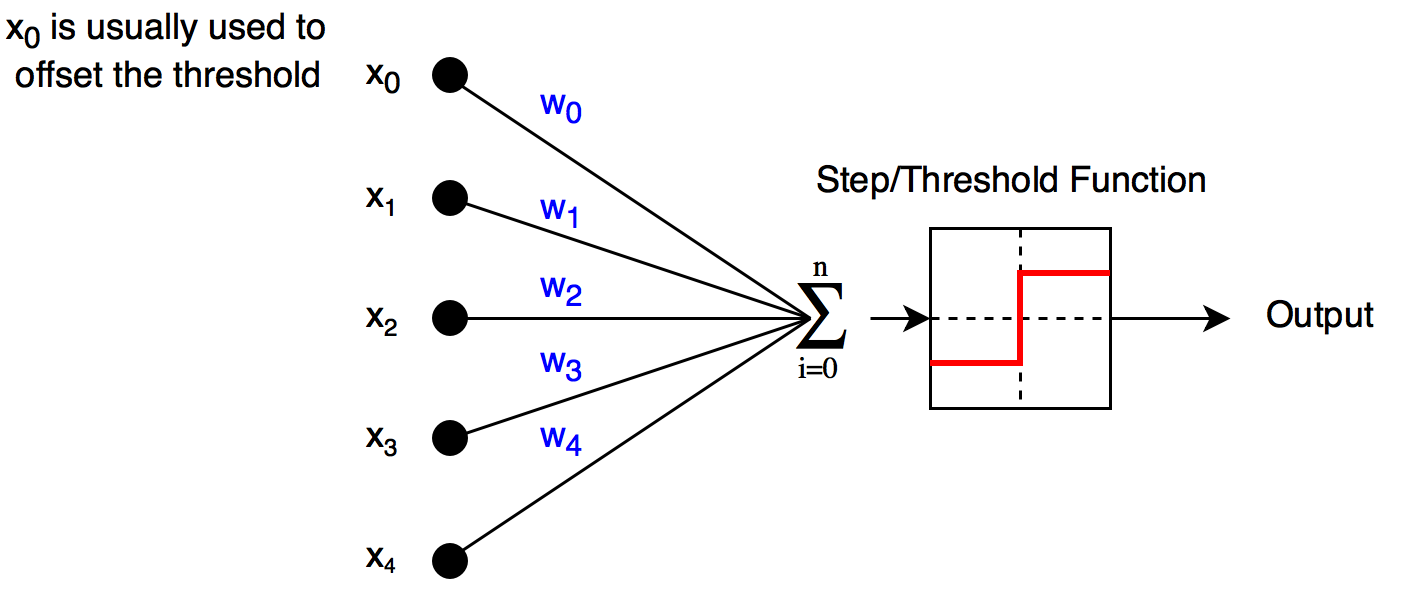
\includegraphics[width=\textwidth]{neuron}
                        \end{figure}
                    
                        \par A neuron has \textit{n} inputs, in this case, 5. Each of the inputs \textit{x\textsubscript{i}} has with it associated a weight, \textit{w\textsubscript{i}}, by which the input is multiplied. This is how different factors are emphasized/diminished, and what is adjusted during "training" of the neuron.
                        
                        \par The inputs, multiplied by their respective weights, are then summed (so x\textsubscript{0}w\textsubscript{0} + x\textsubscript{1}w\textsubscript{1} + ... x\textsubscript{4}w\textsubscript{4} in this particular example), and passed through a threshold function. In the end it looks like:
                        
                        \par \centerline{ {\large output = \(threshold(\sum\limits_{i=0}^n x\textsubscript{i}w\textsubscript{i})\) } }
                        
                        \bigskip
                        
                        \par A threshold function simply fires if the summation is more than some value. So, for example, if the threshold is 0 and if the inputs x\textsubscript{0}w\textsubscript{0} and so on sum to 0 or more, the output will be 1, and 0 otherwise.
                        
                        \par The input x\textsubscript{0} is defined as a constant 1 and the weight w\textsubscript{0} is used to adjust the threshold. If, for instance, w\textsubscript{0} is 0.5, then the entire summation of inputs is essentially shifted to the right by 0.5. If the threshold is set at 0, but it would be preferable to have it at -0.5, we can set w\textsubscript{0} to 0.5. Now, if the inputs, aside from x\textsubscript{0}w\textsubscript{0} sum to -0.5, 0.5 is added (since 1 * 0.5 = 0.5), the entire summation becomes 0, and the threshold function outputs 1.
                    
                        \par That's most of what there is to it. Let us take an example of a neuron which is trying to predict whether a home costs more than 500,000 Euro. The features x\textsubscript{0}, x\textsubscript{1} and so on can be square footage, number of bedrooms and so forth. Different features may be more or less suggestive of the cost of a home, for instance a single square meter increase in area may scarcely affect the price of a home, but an additional bedroom could have a significant impact. Consequently, it would make sense to attach a greater weight w to the number of bedrooms than to the square footage of the property.
                        
                        \par But how would one automatically adjust those weights? The answer, in this particular case, is gradient descent.
                        
                    \subsubsection{Gradient Descent}
                    
                        \par Gradient descent (and it's sibling, gradient ascent) is a simple learning algorithm concerned with utilizing the slope of some abstract space. 
                        
                        \par The intuition is as follows: suppose we formulate a "loss" function \textbf{L} which captures the performance of our neuron, and a set \textbf{S} of houses and their details, as well as whether or not they sold for more than half a million Euro. What \textbf{L} captures is how many of our training samples does our neuron classify correctly.     
                        
                        \par The performance of the loss function depends on the weights we have assigned to each of the inputs, so the function is actually L(W), where W is the set of weights. Suppose there is only a single weight (in order to have a 2-dimensional graph) that we initialize randomly, then the loss function may look like:
                        
                        \begin{figure}[h]
                            \caption{Example loss function.}
                            \centering
                            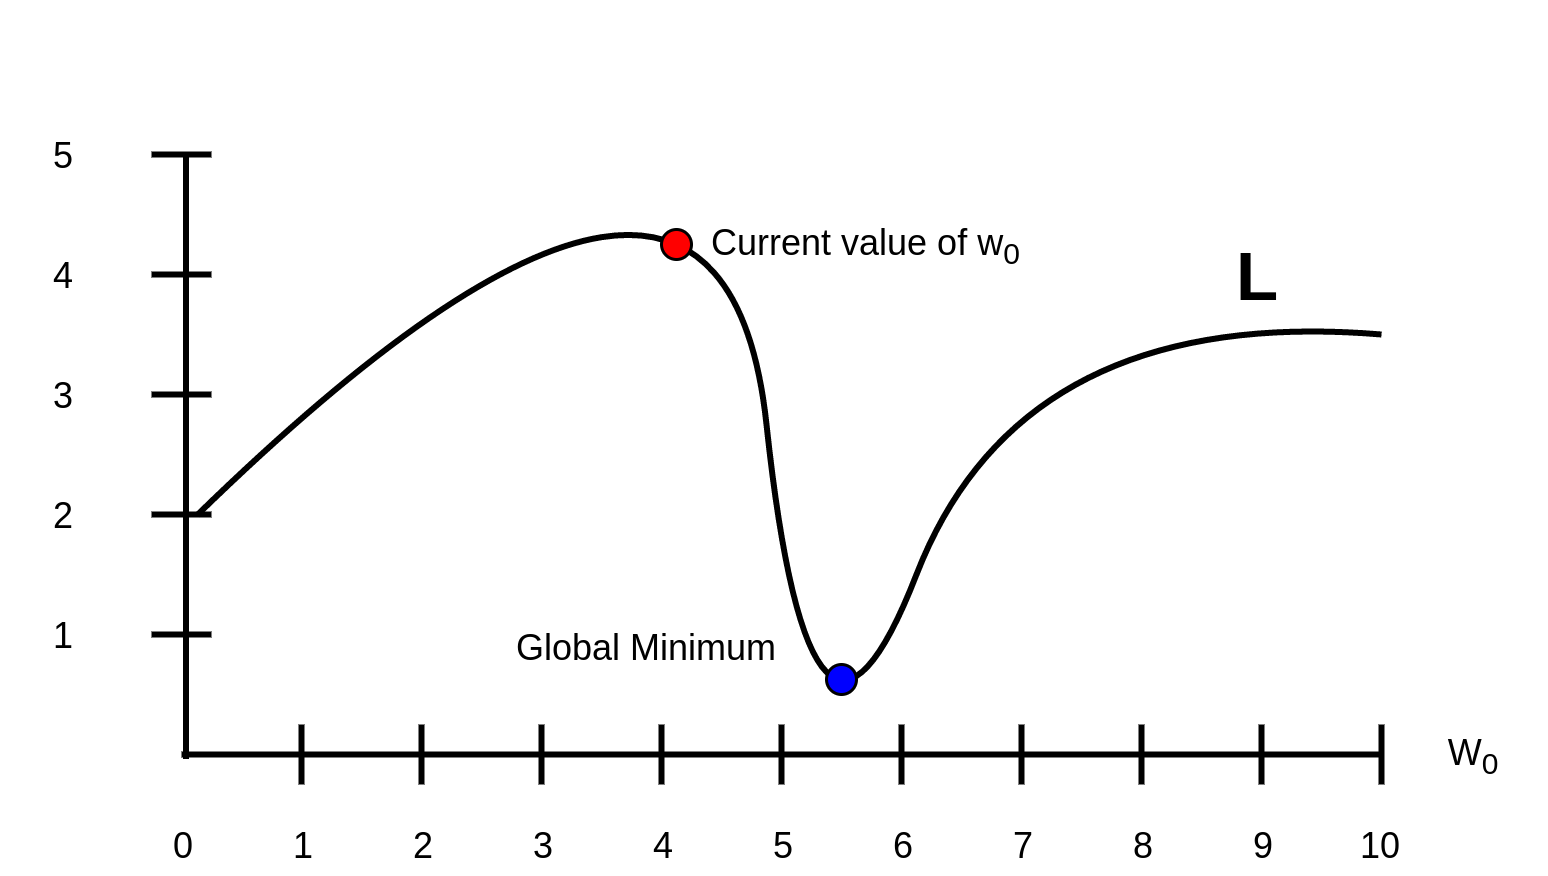
\includegraphics[width=\textwidth]{lossFunction0}
                        \end{figure}
                        
                        \par Now, as we adjust the weight (current red point), the magnitude of our loss function will alter. We can traverse that loss function by changing the weight w. If we change the weight w such that the value loss function decreases, this corresponds to having greater accuracy within our sample, since that is what the loss function captures.
                        
                        \par What gradient descent does is alter the weight in correspondence with the slope of the line. Take our current point, which is fortunately on the cusp of a precipice towards the global minimum of the loss function. The slope at this point is negative, meaning as the value of the variable on the x-axis increases, the value of the variable on the y-axis decreases. We are trying to descend towards the lowest point\footnote{Hence the term gradient descent.}, so a negative slope tells us we should increase the value of w to reduce the value of \textbf{L}.
                        
                        \par When we do so, we might get here (depending on some parameters):
                        
                        \begin{figure}[h]
                            \caption{Adjusted w.}
                            \centering
                            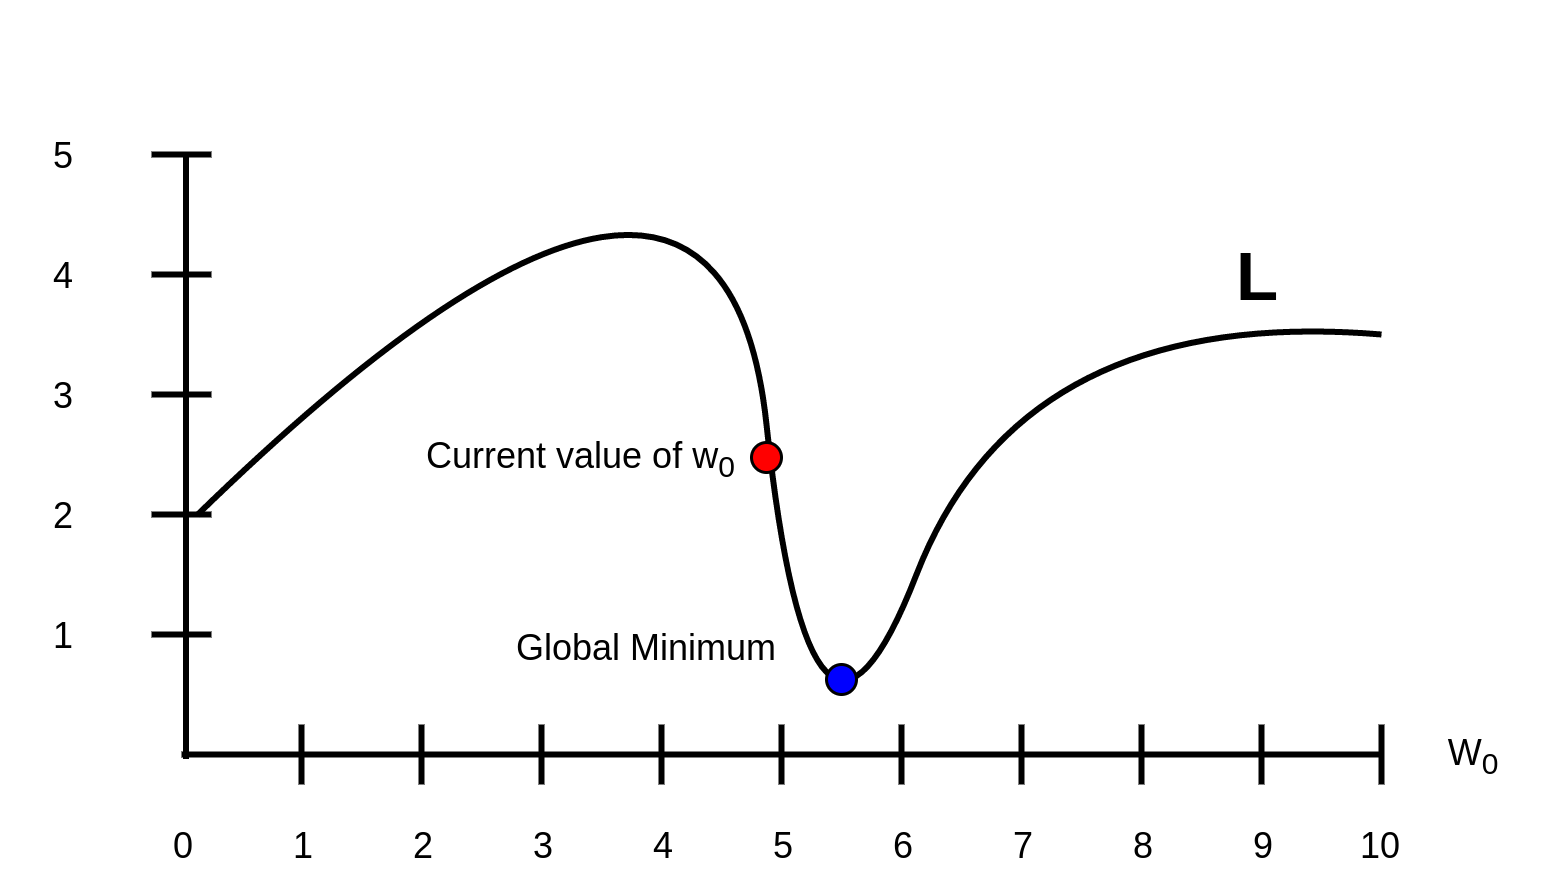
\includegraphics[width=\textwidth]{lossFunction1}
                        \end{figure}
                        
                        \par The iteration then continues until the slope is fount to be ~0 at the global minimum.
                        
                        \par This is a greedy algorithm, and one can see that should w\textsubscript{0} have been initialized to the value of 2 or so, the gradient descent algorithm would have taken it towards the left, rather than the right. Thus, gradient descent is susceptible to "local minima", or little kinks in the graph it may get stuck on. For more details, please see \cite{logisticRegression}\footnote{Relevant part starts at ~ 53:15 minute mark.}.
                        
                        \par Gradient descent is defined as follows:
                        
                        \par {\LARGE w\textsubscript{i} = w\textsubscript{i} - 
                        \(\alpha\)\(\frac{\partial L(W)}{\partial w\textsubscript{i}}\)}
                        
                        \bigskip
                        
                        \par To explain what is going on here. The w\textsubscript{i} is the weight we are currently adjusting, let us say the the weight that will be multiplier of the number of bedrooms in our neuron. The reason for the subscript i is because we may have a whole lot of these, one for each feature, and each of them will be updated differently, since the magnitude of the weights of each of the features will (hopefully) be different. So as we alter the weights, the weight for the number of bedrooms should hopefully increase in larger increments than the weight for the square footage.
                        
                        \par The \(\alpha\) there is the "learning step size". The larger the \(\alpha\), the greater the size of the updates to the weights will be. One may use a constant alpha, or one may reduce it as the number of updates thus far increases and so forth.
                        
                        \par Now that partial derivative, {\Large \(\frac{\partial L(W)}{\partial w\textsubscript{i}}\)}. As You can see, the derivative is of our function L, which should capture the performance of the neuron. The W is the set of all the weights (in our example neuron, this set is of size 5). The L is the function that we are trying to descend or ascend, as the case may be (descend if it is minus \(\alpha\), ascend if plus). Finally, the partial derivative is with respect to the current w\textsubscript{i}, since that is the particular weight that we are currently concerned with. This will all make much more sense with an example.
                        
                        
                    \subsubsection{Training the Neuron}

                        \par All that is left is to apply gradient descent to the neuron and the weights. Unfortunately however, our threshold function is non-continuous and consequently non-differentiable. This is remedied by using a "soft" threshold\cite{mitNeuralNetwork}\footnote{Explained at 25:00 minute mark.}, which makes our neuron diagram look like:
                        
                         \begin{figure}[h]
                            \caption{A simple neuron, with a soft threshold.}
                            \centering
                            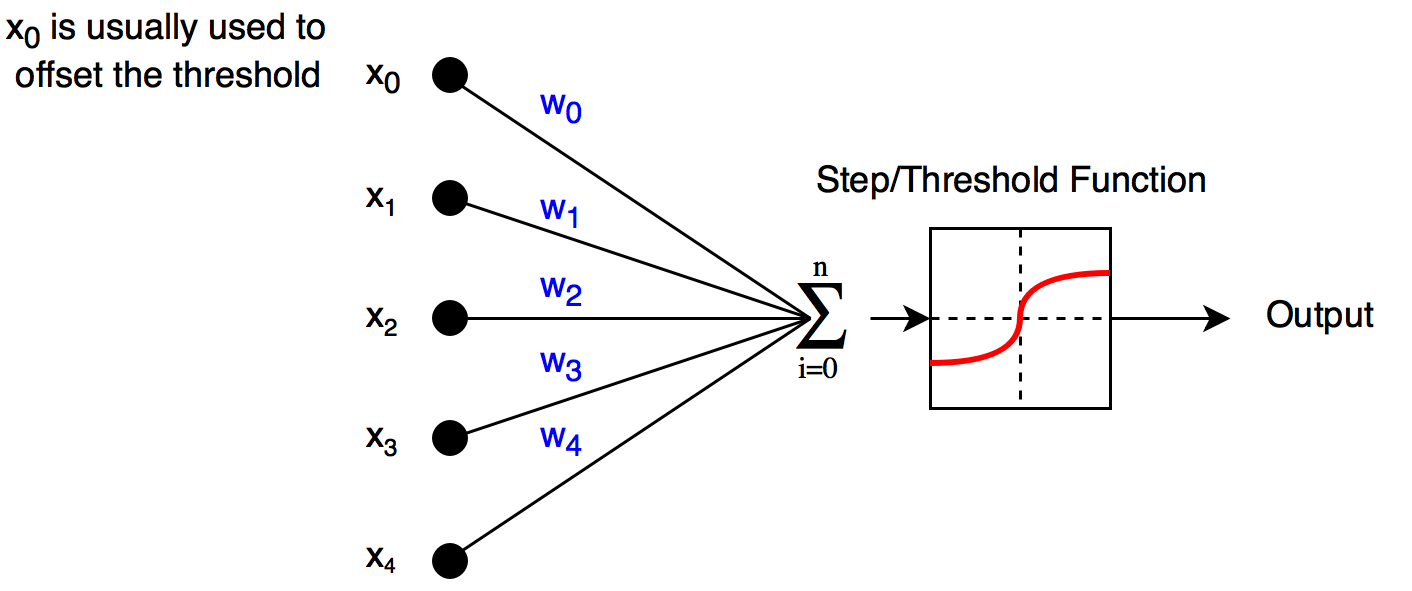
\includegraphics[width=\textwidth]{neuron2}
                        \end{figure}   
                        
                        \par The details of the differentiation can be found at \cite{logisticRegression}\footnote{Explained at the 25:00 minute mark, not a duplicate of above footnote.}, but the intuition should be sufficient for a general understanding.  
                        
                        \newpage
                        
                    \subsubsection{A Network of Neurons, or a Neural Network}                    
                    
                        \par Here is what a neural network looks like visually:
                        
                        \begin{figure}[h]
                            \caption{A neural network.}
                            \centering
                            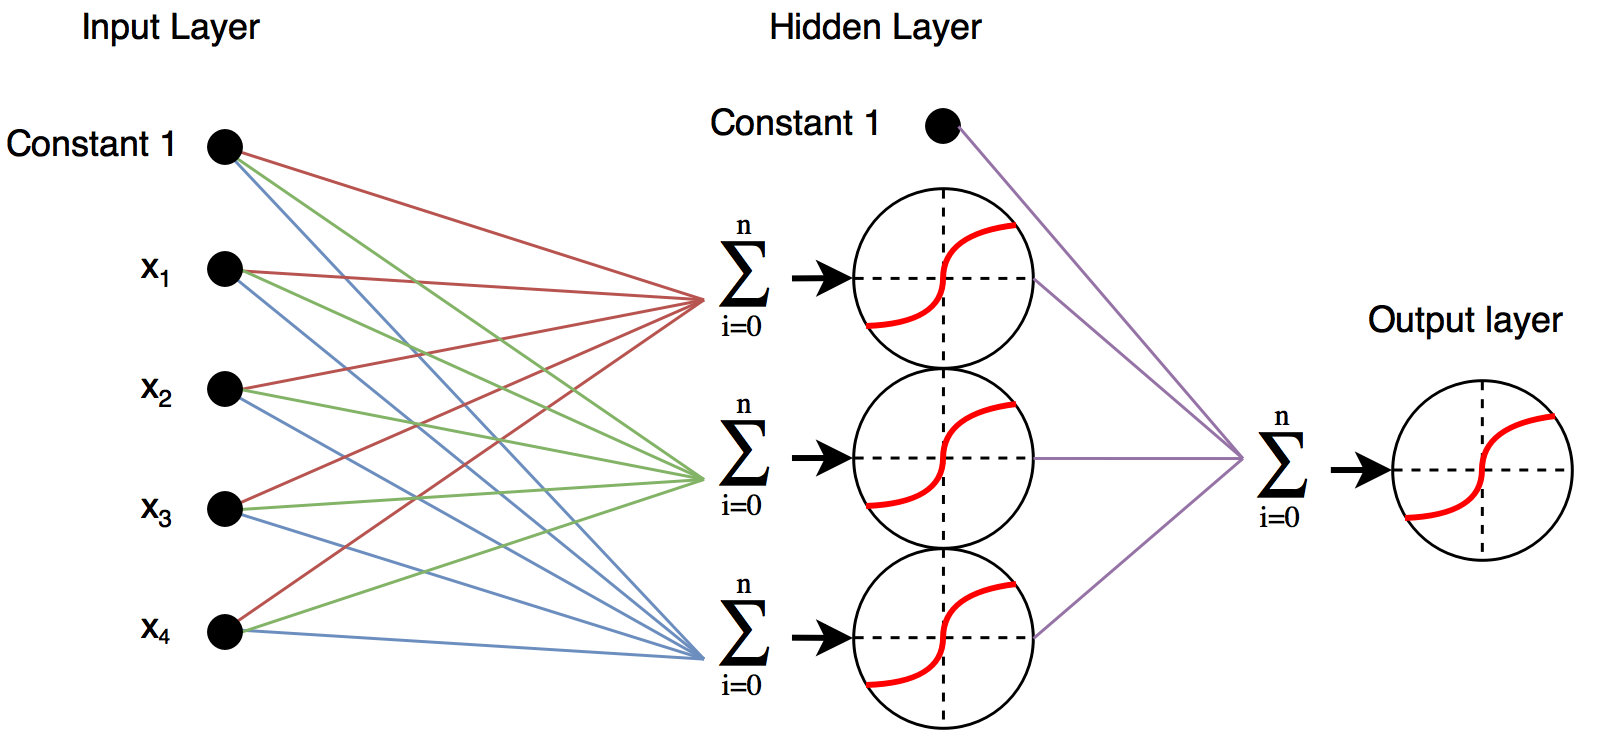
\includegraphics[width=\textwidth]{neuralNetwork}
                        \end{figure}  
                        
                        \par As the name would suggest, it is simply a network of neurons. 
                        
                        \par Note the "hidden" layer, so termed because it is not strictly visible to anyone outside the algorithm. Each of the outputs of the hidden layer have a weight attached to them, just as did the inputs. The network can consist of more than one hidden layer, and the number of neurons in each hidden layer may differ (giving rise to a technique known as autoencoding\cite{autoEncoding}).
                        
                        \par A neural network is trained with gradient descent (either stochastic or batch \cite{caltechNeuralNetwork}). However, a problem arises in the differentiation of the neural network, namely, how does one efficiently find the derivative of the entire neural net with respect to each of the weights w\textsubscript{i}? The change in some weight w\textsubscript{i} affects all downstream neurons, making the derivations very involved\footnote{Explained in much more detail in \cite{mitNeuralNetwork}, 43:00 minute mark.}.
                        
                        \par The answer is an algorithm named "backpropagation". A very broad overview is that by deriving from the output layer backwards (hence back propagation) we can re-use partial derivatives making the differentiation feasible. The algorithm is explained in great detail in \cite{caltechNeuralNetwork}, at the 33:00 minute mark.
                        
                        \par Otherwise, the process by which a neural network is trained is extremely similar to how a single neuron is trained: We are still just optimizing parameters, namely the weights, in order to minimize the value of the loss function, which minimization is done by using gradient descent. The core difference between training a neuron and a neural network is the specialized algorithm for generating partial derivatives with respect to each parameter, backpropagation.
                        
                      
                \newpage                  
                \subsection{Support Vector Machine}
                
                    \subsubsection{Intuition}
                    
                        \par There are two core ideas behind support vector machines: optimal linear separators and kernel functions.
                        
                    \subsubsection{Optimal Linear Separator}
                    
                        \par Picture the following two-dimensional training set:
                        
                        \begin{figure}[h]
                            \caption{A linearly separable set.}
                            \centering
                            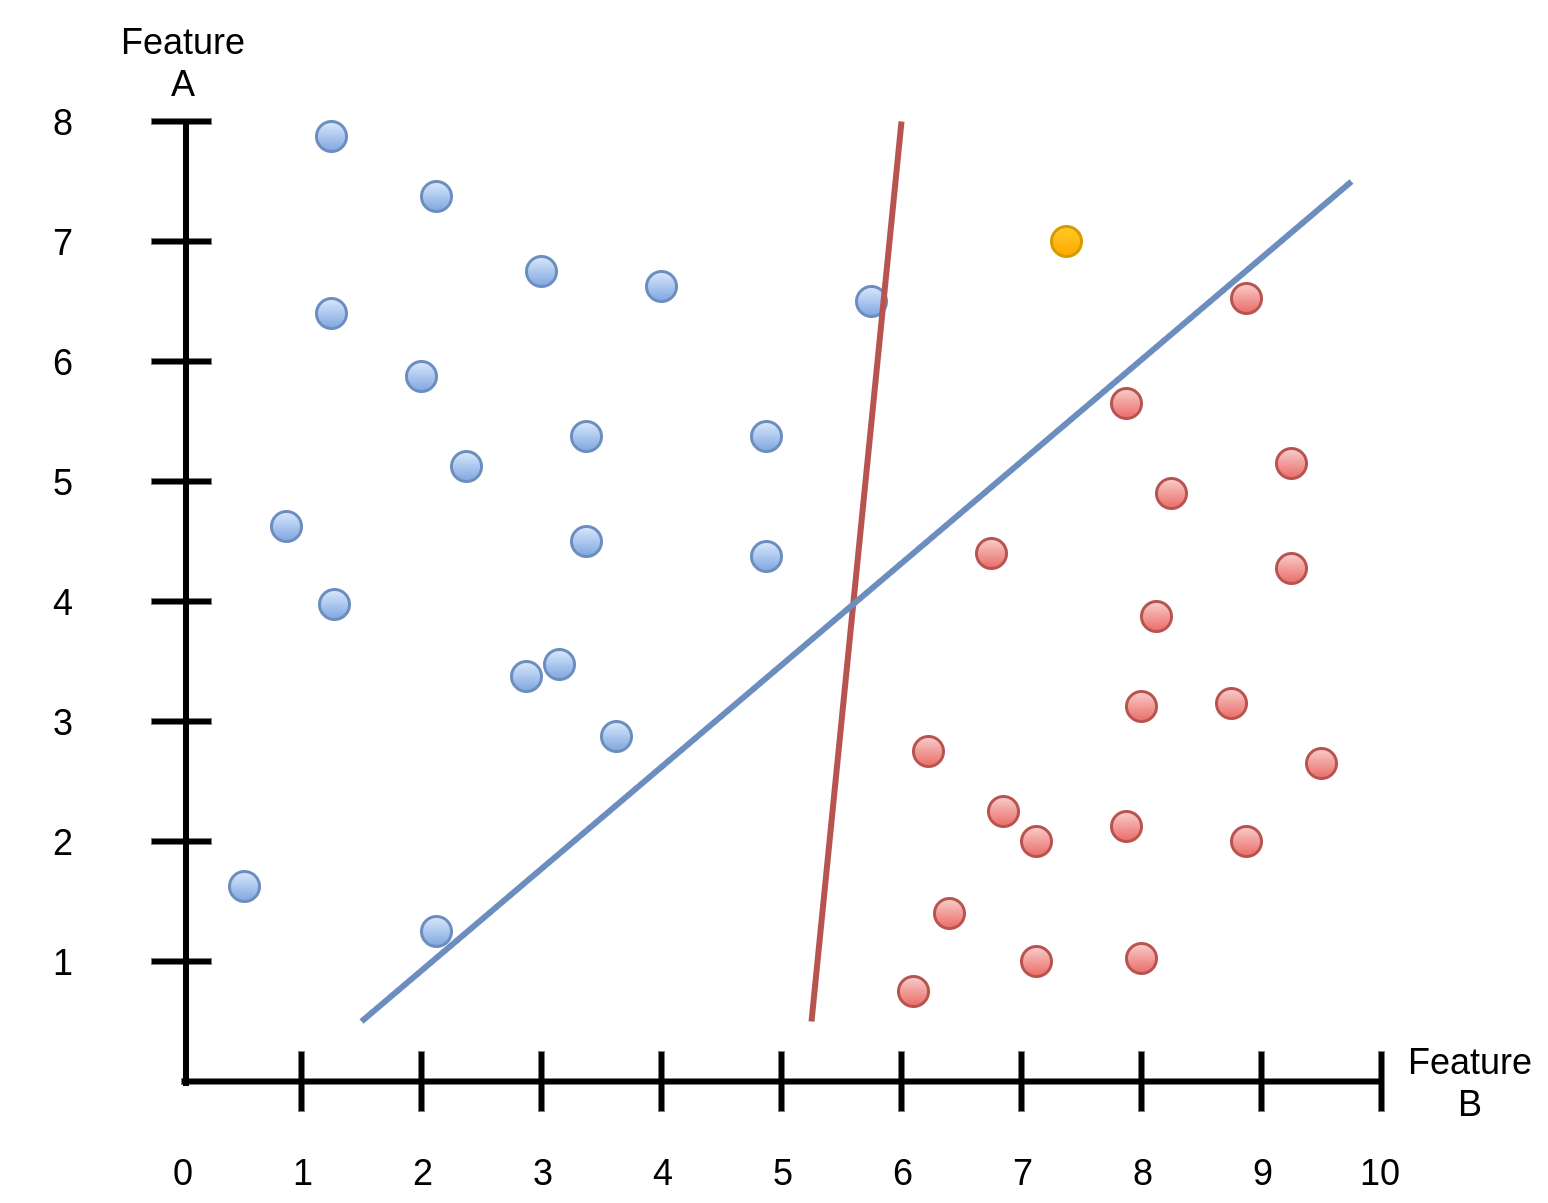
\includegraphics[width=\textwidth]{poorClassifiers}
                        \end{figure}  
                        
                        \par The above is a "linearly separable" set, which simply means that the blue points and the red points can be separated by a straight line\footnote{Which, straight lines are linear functions, hence the term linearly separable.}.
                        
                        \par In the figure, there are two linear separators, the blue and the red. Each gives a different classification to the newly observed sample, which is in gold. Which is the better linear separator? Furthermore, an infinite number of possible separators exist, rather than just the two pictured. How would one go about picking the "best one", and what metric would one use to decide?
                        
                        \par One idea is to try to make a separator that puts as much space between the two clusters (red and blue) as possible, in hopes that that will most faithfully capture the underlying relationship. That separator looks something like:
                        
                        \begin{figure}[h]
                            \caption{A better classifier, allegedly.}
                            \centering
                            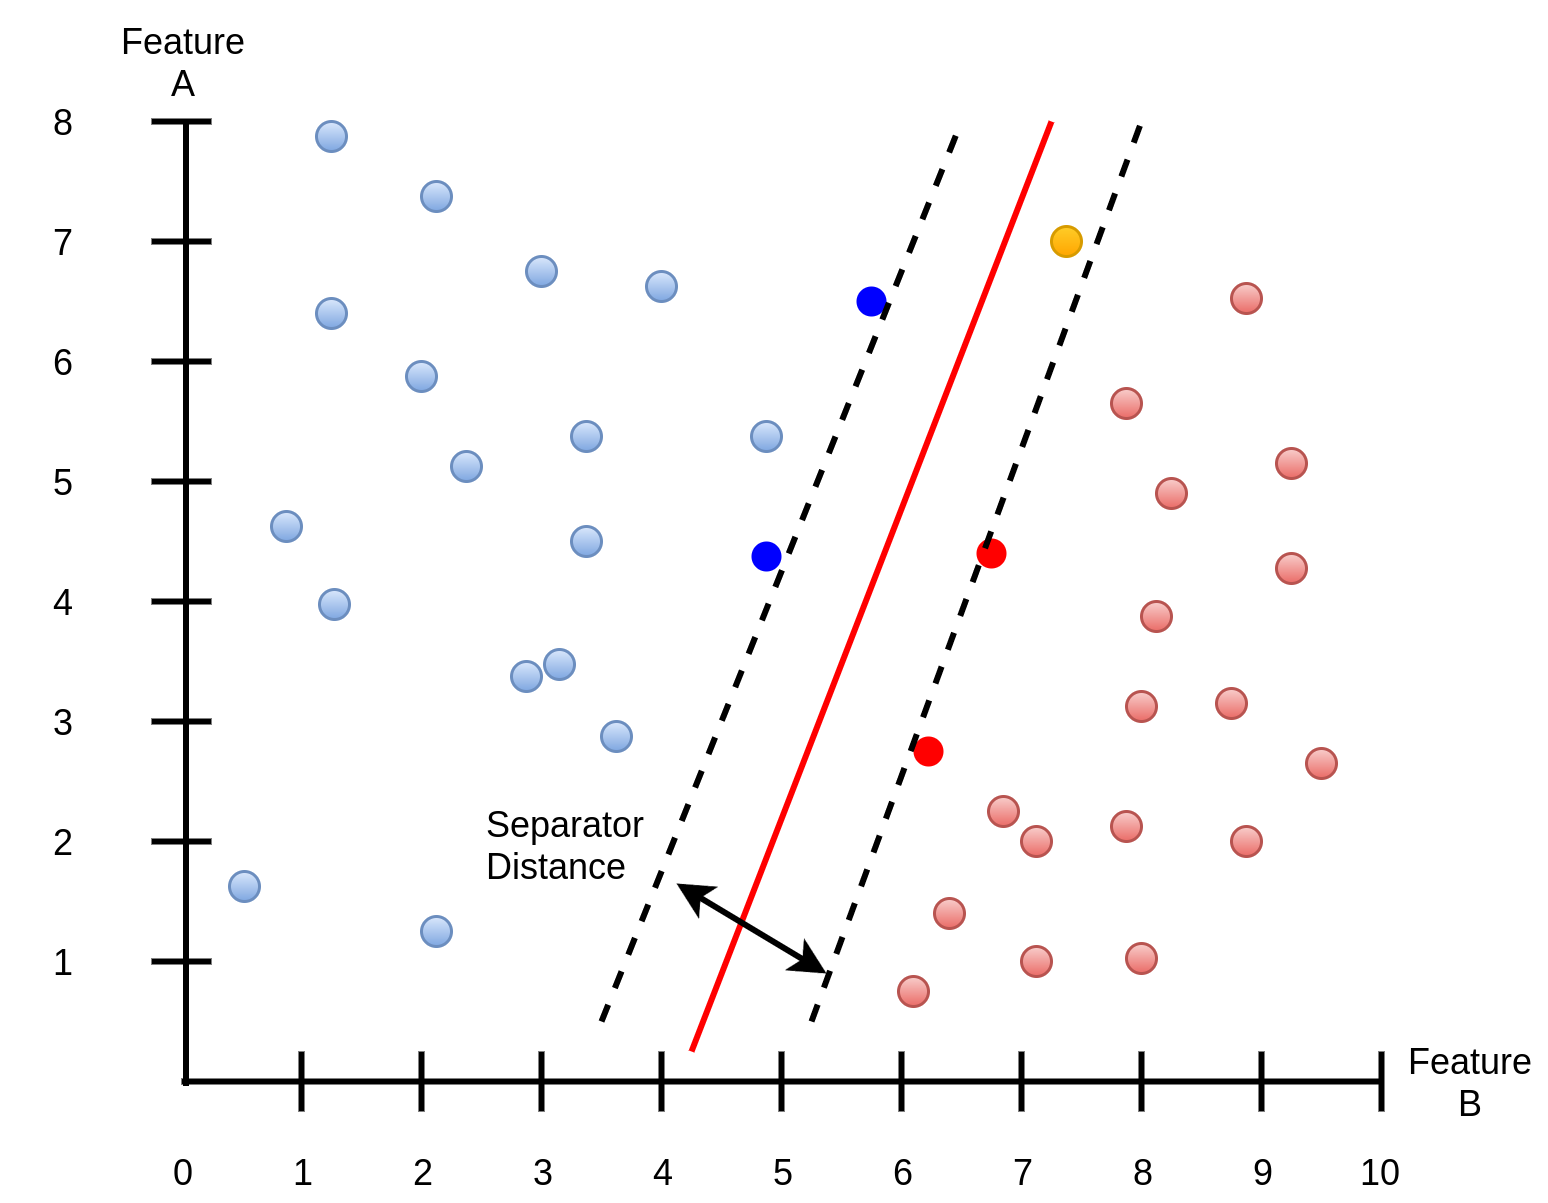
\includegraphics[width=\textwidth]{betterClassifier}
                        \end{figure} 
                        
                        \par To explain some of what is going on there. Picture that the punctuated lines are the edges of a road, and that the red separator in between them marks the center of the road.\footnote{This pedagogical device is from \cite{mitSupportVectorMachine}}
                    
                    
          
    \printbibliography

\end{document}
